\documentclass{article}
\usepackage[utf8]{inputenc}
\usepackage[russian]{babel}
\usepackage{amsfonts}
\usepackage{natbib}
\usepackage{upquote}
\usepackage{datetime}
\usepackage{multicol}
\usepackage{listings}
\usepackage{graphicx}

\setlength{\voffset}{-2cm}
\setlength{\textheight}{700pt}

\title{Численные методы: Домашняя работа}
\author{Группа 4001BV: Карина Пилюшонока}
\date \today

\begin{document}

\maketitle
\newpage
\tableofcontents
\newpage
\section{Расчет индивидуальных коэффициентов для заданий}
Номер группы: 4001BV \\
Номер в журнале: 16 \\
Год посутпления: 2010 \\
Форма обучения: вечерняя

\begin{displaymath} 
  N_{g} = 3 * (4 + 2) + 0 - 1 = 17
\end{displaymath}

\begin{displaymath}
  N_{s} = 16
\end{displaymath}
\section{Метод исключения Гаусса}
\subsection{Подготовка: расчет уравнений для индивидуального задания}
\begin{displaymath}
\left(
  \begin{array}{ccc}
    (N_{g}+4)+5i & -3-4i & 4-4i \\
    -3+2i & 8+(10-N_{s})i & 1+2i \\
    (N_{g}+1)i & N_{s}-10 & N_{s}-N_{g}i
  \end{array}
\right)
=
\left(
  \begin{array}{ccc}
    3+6i\\
    1-(N_{s}-20)i\\
    10i
  \end{array}
\right)
\end{displaymath}
После отброса мнимой части из уравнений получаем следующие коэффициенты для
уравнений:
\begin{displaymath}
\left(
  \begin{array}{ccc}
    21 x_{1} & -3 x_{2} & 4 x_{3} \\
    -3 x_{1} & 8 x_{2} & 1 x_{3} \\
    0 & 6 x_{2} & 16 x_{3}
  \end{array}
\right)
=
\left(
  \begin{array}{ccc}
    3\\
    1\\
    0
  \end{array}
\right)
\end{displaymath}

\subsection{Прямой ход Гаусса}
итерация: 1
\begin{displaymath}
\left(
  \begin{array}{ccc}
    21 x_{1} & -3 x_{2} & 4 x_{3} \\
    0 & 7.571428571428571 x_{2} & 1.5714285714285714 x_{3} \\
    0 & 6 x_{2} & 16 x_{3}
  \end{array}
\right)
=
\left(
  \begin{array}{ccc}
    3\\
    1.4285714285714286\\
    0
  \end{array}
\right)
\end{displaymath}
итерация: 2
\begin{displaymath}
\left(
  \begin{array}{ccc}
    21 x_{1} & -3 x_{2} & 4 x_{3} \\
    0 & 7.571428571428571 x_{2} & 1.5714285714285714 x_{3} \\
    0 & 0 & -14.754716981132075 x_{3}
  \end{array}
\right)
=
\left(
  \begin{array}{ccc}
    3\\
    1.4285714285714286\\
    -1.1320754716981134
  \end{array}
\right)
\end{displaymath}

\subsection{Результат обратного хода Гаусса}
\begin{displaymath}
\mathbf{X} =
\left( \begin{array}{ccc}
  0.1867007672634271 \\
  0.20460358056265987 \\
  -0.07672634271099746 
\end{array} \right)
\end{displaymath}

\subsection{Проверка}
yравнение 1:
\begin{displaymath}
  21 * 0.1867007672634271 -3*0.20460358056265987 + 4 * (-0.07672634271099746) = 3
\end{displaymath}
yравнение 2:
\begin{displaymath}
  -3 * 0.1867007672634271 + 8*0.20460358056265987 + 1 * (-0.07672634271099746) = 1.0000000000000002
\end{displaymath}
yравнение 3:
\begin{displaymath}
  0*0.1867007672634271 + 6*0.20460358056265987 + 16 * (-0.07672634271099746) = 0
\end{displaymath}

\subsubsection{Невязка}
yравнение 1:
\begin{displaymath}
  3-3 = 0  
\end{displaymath}
yравнение 2:
\begin{displaymath}
  1.0000000000000002 - 1 = 2.220446049250313e-16
\end{displaymath}
yравнение 3:
\begin{displaymath}
  0 - 0 = 0
\end{displaymath}

\section{Методы приближения функции. Интерполяция и аппроксимация}

\subsection{Подготовка: расчет узлов}
\begin{table}[!h]
  \begin{tabular}{|l|l|l|l|l|}
  \hline
  \bfseries x & -1 & $N_{g}$   & 6 & 10\\
  \hline
  \bfseries y &  1 & $N_{s}-5$ & 8 & -2\\
  \hline
  \end{tabular}
\end{table}
При подстановке $N_{g}$ и $N_{s}$ получим следующий набор узлов:
\begin{table}[!h]
  \begin{tabular}{|l|l|l|l|l|}
  \hline
  \bfseries x & -1 & $17$ & 6 & 10\\
  \hline
  \bfseries y &  1 & $11$ & 8 & -2\\
  \hline
  \end{tabular}
\end{table}
 
\subsection{Полином Лагранжа}
\subsection{Полином Ньютона}
\subsection{Метод наименьших квадратов}
\subsection{Графическое отображение}

\section{Методы численного интегрирования и дифференцирования}
\subsection{Метод прямоугольников}
\subsection{Метод трапеций}
\subsection{Метод Симпсона}
\subsection{Квадратура Гаусса}

\section{Решение нелинейного уравнения}
\subsection{Подготовка: создание уравнения, вспомогательные элементы}

\begin{displaymath}
  \begin{array}{ccc}
    f(x) = x / sin^2(3x)  \\
    f'(x) = (1 - 6x cos(3 x) / sin(3 x)) 1/sin^2(3 x)\\
    f''(x) = 6/sin^4(3x) * (6x - sin(6x) + 3x * cos(6x))
  \end{array}
\end{displaymath}

\begin{displaymath}
  \begin{array}{ccc}
    f(x) = N_{g}  \\
    x / sin^2(3x) = 17 \\
    x / sin^2(3x) - 17 = 0 \\
  \end{array}
\end{displaymath}

Точность: $\varepsilon = 0.0001$

Интервал для поиска корней: [0.1; 1]

\subsection{Метод бисекции}

Итерация: 1
\begin{displaymath}
  x: 0.55, ab = [0.1, 1];
\end{displaymath}
итерация: 2
\begin{displaymath}
  x: 0.775, ab = [0.55, 1];
\end{displaymath}
итерация: 3
\begin{displaymath}
  x: 0.8875, ab = [0.775, 1];
\end{displaymath}
итерация: 4
\begin{displaymath}
  x: 0.94375, ab = [0.8875, 1];
\end{displaymath}
итерация: 5
\begin{displaymath}
  x: 0.971875, ab = [0.94375, 1];
\end{displaymath}
итерация: 6
\begin{displaymath}
  x: 0.9578125, ab = [0.94375, 0.971875].
\end{displaymath}

Результат: $x = 0.966876220703125$, за 14 итераций.

\subsection{Метод хорд}
Условие сходимости метода: 
\begin{displaymath}
  \begin{array}{ccc}
    f(1) = x / sin^2(3x) = 33.213768360408736 \\
    f''(1) = 6/sin^4(3x) * (6x - sin(6x) + 3x * cos(6x)) = 138576.26831776567
  \end{array}
\end{displaymath}
- знак не меняется, значит метод применим.\\
Итерация: 1
\begin{displaymath} 
  x: 0.3908054983496253, ab = [0.1, 1]
\end{displaymath}
итерация: 2
\begin{displaymath}
  x: 0.5933240899277314, ab = [0.3908054983496253, 1]
\end{displaymath}
итерация: 3
\begin{displaymath}
  x: 0.7276420688960742, ab = [0.5933240899277314, 1]
\end{displaymath}
итерация: 4
\begin{displaymath}
  x: 0.8158659960100441, ab = [0.7276420688960742, 1]
\end{displaymath}
итерация: 5
\begin{displaymath}
  x: 0.8731678144064535, ab = [0.8158659960100441, 1]
\end{displaymath}
итерация: 6
\begin{displaymath}
  x: 0.9098002888447452, ab = [0.8731678144064535, 1]
\end{displaymath}

Результат: $x = 0.9668512818566148$, за 18 шагов.

\subsection{Метод Ньютона}
\begin{displaymath}
  x_{0}: 0.55;
\end{displaymath}
Итерация: 1
\begin{displaymath}
  x: 13.50135782145894  delta: 12.95135782145894;
\end{displaymath}
итерация: 2
\begin{displaymath}
  x: 13.451261598353025  delta: 0.05009622310591588;
\end{displaymath}
итерация: 3
\begin{displaymath}
  x: 13.387853446812523  delta: 0.06340815154050183;
\end{displaymath}
итерация: 4
\begin{displaymath}
  x: 13.321324383604663  delta: 0.06652906320785945;
\end{displaymath}
итерация: 5
\begin{displaymath}
  x: 13.272783216385665  delta: 0.04854116721899793;
\end{displaymath}
итерация: 6
\begin{displaymath}
  x: 13.254786613462766  delta: 0.017996602922899285.
\end{displaymath}

Результат: $x = 13.252873093705627$, за 8 итераций.
\subsubsection{Метод Ньютона: пояснение результата}
  Метод Ньютона, при начальном $x_{0} = 0.55$ не сходится (см.
  Рис.\ref{equ_newton_img}).
  \begin{figure}[b]
    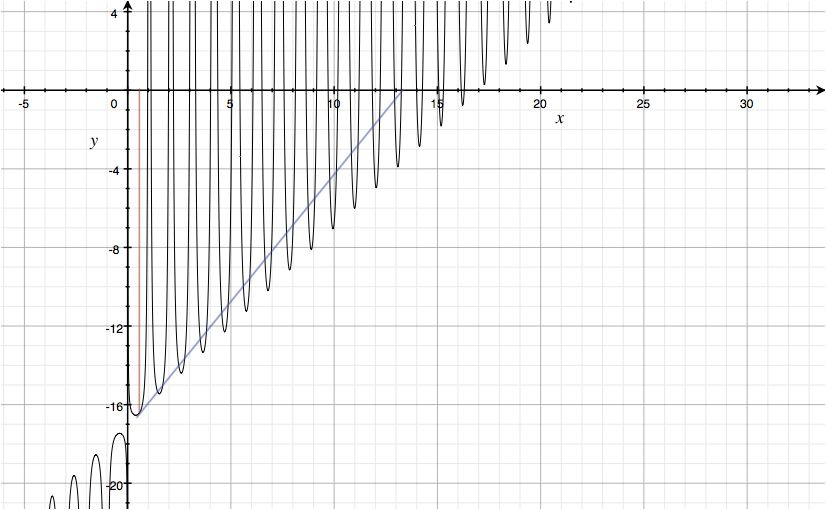
\includegraphics[width=13cm]{equations_newton.png}
    \caption{Первые шаги поиска корня методом Ньютона для функции $x/sin^2(3x)
    - 17$}
    \label{equ_newton_img}
  \end{figure}

\subsection{Метод простых итераций}

\section{Решение линейного дифференциального уравнения 2-го порядка}
\subsection{Метод Рунге-Кутта}

\section{Разложение периодической функции в ряд Фурье}


\end{document}
